\begin{ex}
 (Ufla) Um problema clássico de combinatória é calcular o número de maneiras de se colocar bolas iguais em caixas diferentes. Calcule o número de maneiras de se colocar 7 bolas iguais em 3 caixas diferentes, sem que nenhuma caixa fique vazia.
   \begin{sol}
       \phantom{A}  \\ 

     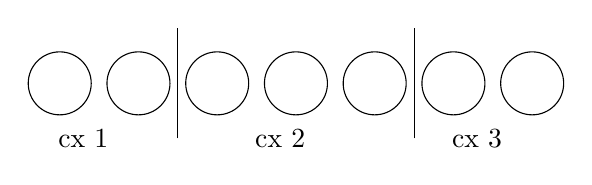
\begin{tikzpicture}
       \draw (0,0) circle [radius=0.4]; 
       \draw (1,0) circle [radius=0.4];
       \draw (2,0) circle [radius=0.4];
       \draw (3,0) circle [radius=0.4];
       \draw (4,0) circle [radius=0.4];
       \draw (5,0) circle [radius=0.4];
       \draw (6,0) circle [radius=0.4];
       \draw (1.5,-.7)--(1.5,.7);
       \draw (4.5,-.7)--(4.5,.7);
       \node at (0.3,-0.7) {cx 1};
       \node at (2.8,-0.7) {cx 2};
       \node at (5.3,-0.7) {cx 3};
     \end{tikzpicture}
     \\
     Como temos 7 bolas, existem 6 espaços entre as bolas. Temos também 2 separadores entre as bolas, logo o problema se resume em $\mathrm{C}_{6,2}=15$
   \end{sol}
\end{ex}